\section{Eksperimentinis tyrimas}\label{sec:experiment}

\subsection{Tyrimo aprašymas}
Naudodami \refFramework{MalGAN} \glswhat{framework} paruošime
\glswhat{adversarial} ir apskaičiuosime jų efektyvumą prieš komercinius
detektorius.

\subsubsection{\acs{gan} įgyvendinimas}

Naudosime \href{https://github.com/ZaydH/MalwareGAN}{viešai \textit{Github}
    platformoje paskelbtą\footnote{https://github.com/ZaydH/MalwareGAN}}
\textit{MalGAN} karkaso \acs{ml} modelio įgyvendinimą.

\begin{equation}
    L_{D}= -\mathbb{E}_{x\in BB_{Benign}}\log\left(1-D_{\theta_{d}}(x)\right)\\-\mathbb{E}_{x\in BB_{Malware}}\log D_{\theta_{d}}\left(x\right).\label{eq:LD}
\end{equation}

\begin{equation}
    L_G= \mathbb{E}_{m \in S_{Malware},z \sim p_{\mathrm{uniform} \left[0,1\right) }} \log D_{\theta_d} \left(G_{\theta_g} \left(m,z\right) \right)\label{eq:LG}
\end{equation}

\ref{eq:LD}-oje ir \ref{eq:LG}-oje lygtyse atitinkamai pateikiamos \textit{MalGAN} diskriminatoriaus ir generatoriaus nuostolių funkcijos. Šiose lygtyse naudojamų simbolių prasmės paaiškinimas pateikiamas \ref{tab:eq_explain}-oje lentelėje.

\begin{table}[h]
    \begin{small}
        \begin{center}
            \begin{tabular}[c]{l|p{0.75\textwidth}}
                Simbolis       & Prasmė                                                                                                                                           \\
                \midrule
                $BB_{Benign}$  & Požymių vektorių, kuriuos \enquote{juodos dėžės} detektorius klasifikuoja kaip \textbf{nekenksmingus}, aibė                                      \\

                $BB_{Malware}$ & Požymių vektorių, kuriuos \enquote{juodos dėžės} detektorius klasifikuoja kaip \textbf{kenksmingus}, aibė                                        \\

                $S_{Malware}$  & Tikrų kenkėjiškų programų požymių vektorių aibė                                                                                                  \\

                $D_{\theta_d}$ & Diskriminatorius su $\theta_d$ svoriais ($D_{\theta_d}: \set{0,1}^{n_m} \rightarrow [0,1], \; n_m \in \mathbb{N}$)                               \\

                $G_{\theta_g}$ & Generatorius su $\theta_g$ svoriais ($G_{\theta_g}: \set{0,1}^{n_m} \times {[0,1]}^{n_z} \rightarrow \set{0,1}^{n_m}, \; n_m, n_z \in \mathbb{N}$) \\

                $z$            & Triukšmo vektorius                                                                                                                               \\

            \end{tabular}
        \end{center}
        \caption{\textit{MalGAN} nuostolių funkcijų formulėse naudojamų simbolių paaiškinimas}\label{tab:eq_explain}
    \end{small}
\end{table}


\subsubsection{\acs{gan} mokymosi duomenys} Mokymuisi naudosime \textit{EMBER}
\cite{andersonEMBEROpenDataset2018a} duomenų rinkinį. Mokymosi aibė susideda iš
$2000$ programų požymių (\textit{API} vardų iš \textit{ImportTable} \acs{pe}
formato failo sekcijos). Aibė subalansuota -- joje yra po $1000$ kenkėjiškų ir
nekenkėjiškų programų požymių. Mokymosi etapui taip pat taikysime mokymosi /
validacijos skaidinį santykiu $4:1$.

\subsubsection{\Glswhom{framework} parametrai}

Tyrimo metu atlikti 2 eksperimentai (\textbf{E-1} ir \textbf{E-2}), kuriems
parinkti \ref{tab:experiment:params}-oje lentelėje aprašyti parametrai.
\textbf{E-1} atitinka \textit{MalGAN} straipsnyje
\cite{huGeneratingAdversarialMalware2017} aprašytą eksperimentą, \textbf{E-2}
-- eksperimentas su autoriaus parinktais parametrais siekiant padidinti atakų
efektyvumą.

\begin{table}[h]
    \begin{tabular}{|l|l|l|}
        \textbf{Parametras}                                                   & \textbf{E-1} & \textbf{E-2}          \\
        \midrule
        Dvejetainio požymių vektoriaus $M$ dimensija                          & 160          & $10000$               \\
        \enquote{Triukšmo} vektoriaus $Z$ dimensija                           & 10           & $100$                 \\
        Neuronų skaičius generatoriaus \enquote{paslėptuose} sluoksniuose     & 256          & $100, 256, 512, 1024$ \\
        Neuronų skaičius diskriminatoriaus \enquote{paslėptuose} sluoksniuose & 256          & $256, 256$            \\
        Diskriminatoriaus mokymosi greitis                                    & $10^{-3}$    & $4\cdot 10^{-4}$      \\
        Generatoriaus mokymosi greitis                                        & $10^{-3}$    & $10^{-6}$             \\
    \end{tabular}
    \caption{Eksperimentuose naudoti \acs{ml} modelio parametrai}\label{tab:experiment:params}
\end{table}

\subsubsection{Realių kenkėjiškų programų rinkinys}\label{sec:experiment:virusshare}
Atakoms naudosime realias kenkėjiškas \acs{pe} formato programas iš
\href{https://virusshare.com/}{\textit{VirusShare}\footnote{https://virusshare.com/}}.
Duomenų rinkinį sudaro $100$ kenkėjiškų programų.

\subsubsection{Komerciniai detektoriai}
Tiek originalias, tiek modifikuotas (\acs{ae}) kenkėjiškas programas
patikrinsime su
\href{https://www.virustotal.com}{\textit{VirusTotal}\footnote{https://www.virustotal.com}}
-- paslauga, kuri agreguoja daugiau nei $70$ komercinių kenkėjiškų programų
detektorių.

\clearpage
\subsection{Mokymosi etapas}

Specifinis \refFramework{MalGAN} mokymosi etapas yra tokia seka:
\begin{enumerate}
    \item Išmokomas \enquote{juodos dėžės} modelis (šiuo atveju pasirinktas
          \enquote{atsitiktinio miško} (\angl{random forest}) modelis).
    \item Mokoma pagal bendrą seką (aptartą \ref{sec:literature:gan}), kurioje:
          \begin{itemize}
              \item Praleidžiamas originalios programos perturbacijos žingsnis (diskriminatoriui
                    iškart perduodamas \acs{ae} požymių vektorius).
              \item Generatorius ir diskriminatorius mokomi kartu, kadangi diskriminatorius turi
                    naudoti generatoriaus sugeneruotus \acs{ae}, o generatoriaus nuostolių funkcija
                    priklauso nuo diskriminatoriaus išvesties. Šis žingsnis pavaizduotas
                    \ref{fig:experiment:learning:combined}-ame pav.
          \end{itemize}
\end{enumerate}

\begin{figure}[h]
    \begin{small}
        \begin{center}
            \begin{subfigure}[t]{0.5\textwidth}
                \centering
                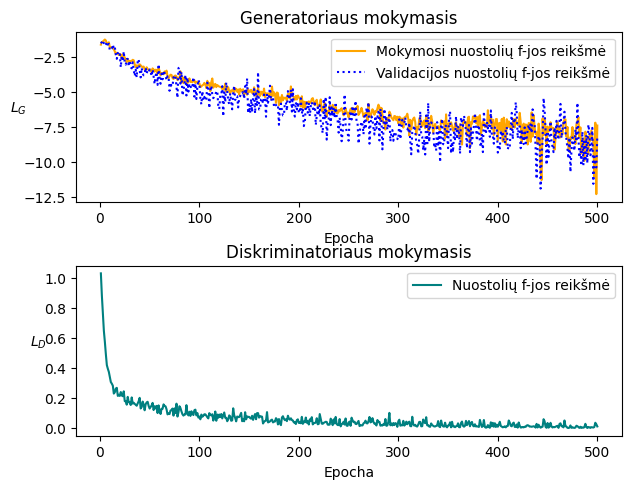
\includegraphics[width=\textwidth]{img/learning_paper.png}
                \caption{\textbf{E-1}}\label{fig:experiment:learning:paper}
            \end{subfigure}
            \hfill
            \begin{subfigure}[t]{0.48\textwidth}
                \centering
                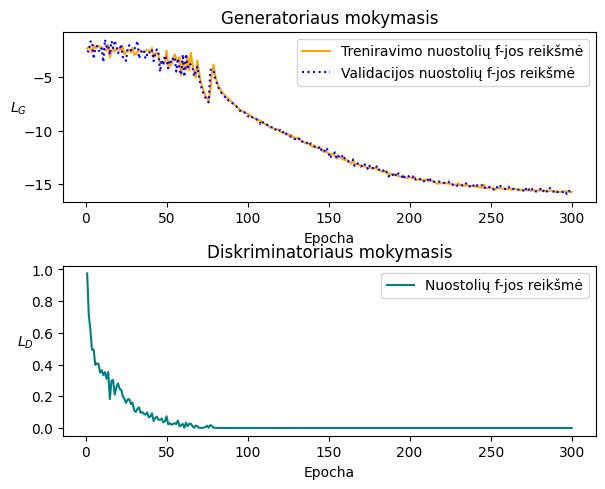
\includegraphics[width=\textwidth]{img/learning.png}
                \caption{\textbf{E-2}}\label{fig:experiment:learning}
            \end{subfigure}
        \end{center}
    \end{small}
    \caption{\textit{MalGAN} generatoriaus ir diskriminatoriaus nuostolių funkcijų reikšmės mokymosi etape}\label{fig:experiment:learning:combined}
\end{figure}

\clearpage
\subsection{Varžymosi principais pagrįstos atakos prieš komercinius detektorius}

Naudodami mokymosi etape išmokytą \acs{ml} modelį ir
\ref{sec:experiment:virusshare} aptartą duomenų rinkinį, sugeneruosime \acs{ae}
ir palyginsime, kiek komercinių detektorių aptinka originalias programas
($N_{orig}$) ir kiek obfuskuotas pagal \textit{MalGAN} karkasą ($N_{adv}$).

Atakų efektyvumą $\mu$ skaičiuosime remiantis Zhong et~al. pasiūlyta formule
$\mu' = \frac{N_{orig} - N_{adv}}{N_{orig}}$
\cite{zhongMalFoxCamouflagedAdversarial2024}. Eksperimentuose galimi atvejai,
kai originalią programą aptinka mažesnis detektorių kiekis, nei obfuskuotą
($N_{orig} < N_{adv}$). Tokiais atvejais $\mu' < 0$. Kadangi neigiamas atakos
efektyvumas neturi prasmės, laikome, jog atvejais, kai $\mu' < 0$ ataka nėra
efektyvi (t.~y. jos efektyvumas lygus $0$) $\implies$ $\mu = \max{(\mu', 0)}$.

Atakų efektyvumų pasiskirstymas pavaizduotas \ref{fig:experiment:mu_dist}-ame
pav., tarpiniai rezultatai ($N_{orig}$ ir $N_{adv}$), naudojami pasiskirstymų
skaičiavimui pateikiami \ref{fig:experiment:det_dist}-ame pav.
(\ref{app:experiment}-ame priede).

\begin{figure}[h]
    \begin{small}
        \begin{center}
            \begin{subfigure}[t]{0.48\textwidth}
                \centering
                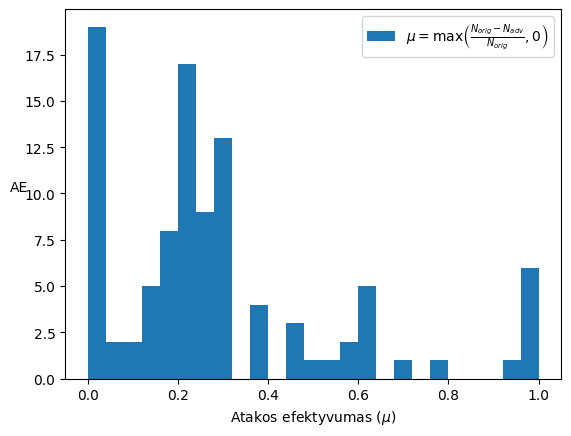
\includegraphics[width=\textwidth]{img/mu_distribution_paper.png}
                \caption{\textbf{E-1}}
            \end{subfigure}
            \hfill
            \begin{subfigure}[t]{0.48\textwidth}
                \centering
                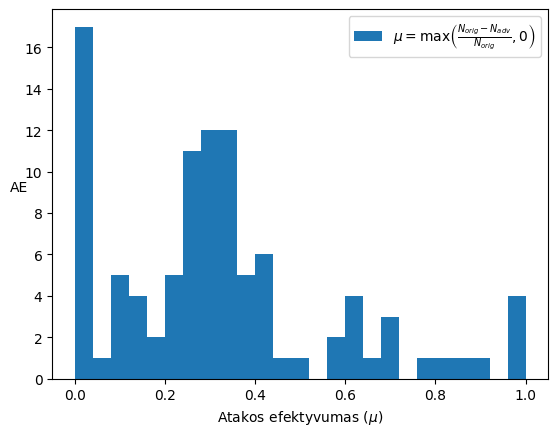
\includegraphics[width=\textwidth]{img/mu_distribution.png}
                \caption{\textbf{E-2}}
            \end{subfigure}
        \end{center}
        \caption{\Glswhose{adversarial} efektyvumo prieš komercinius detektorius pasiskirstymas}\label{fig:experiment:mu_dist}
    \end{small}
\end{figure}

Tyrimo apibendrinimui \ref{tab:experiment:stats}-oje lentelėje pateikiamos
abiejų eksperimentų statistikos, apskaičiuotos iš
\ref{fig:experiment:mu_dist}-ame pav. vaizduojamų duomenų įtraukiant ir
neefektyvias atakas (kai $\mu = 0$).

\begin{table}[h]
    \centering
    \begin{tabular}{l|l|l}
                                                   & \textbf{E-1} & \textbf{E-2} \\
        \midrule
        \textbf{Efektyvumo vidurkis ($\bar{\mu}$)} & $28,89 \; \%$   & $26,85 \; \%$   \\
        \textbf{Standartinis nuokrypis ($\sigma$)} & $26,31 \; \%$   & $18,97 \; \%$   \\
    \end{tabular}
    \caption{Eksperimentų statistikos}\label{tab:experiment:stats}
\end{table}
